\documentclass[twoside]{book}

% Packages required by doxygen
\usepackage{fixltx2e}
\usepackage{calc}
\usepackage{doxygen}
\usepackage[export]{adjustbox} % also loads graphicx
\usepackage{graphicx}
\usepackage[utf8]{inputenc}
\usepackage{makeidx}
\usepackage{multicol}
\usepackage{multirow}
\PassOptionsToPackage{warn}{textcomp}
\usepackage{textcomp}
\usepackage[nointegrals]{wasysym}
\usepackage[table]{xcolor}

% Font selection
\usepackage[T1]{fontenc}
\usepackage[scaled=.90]{helvet}
\usepackage{courier}
\usepackage{amssymb}
\usepackage{sectsty}
\renewcommand{\familydefault}{\sfdefault}
\allsectionsfont{%
  \fontseries{bc}\selectfont%
  \color{darkgray}%
}
\renewcommand{\DoxyLabelFont}{%
  \fontseries{bc}\selectfont%
  \color{darkgray}%
}
\newcommand{\+}{\discretionary{\mbox{\scriptsize$\hookleftarrow$}}{}{}}

% Page & text layout
\usepackage{geometry}
\geometry{%
  a4paper,%
  top=2.5cm,%
  bottom=2.5cm,%
  left=2.5cm,%
  right=2.5cm%
}
\tolerance=750
\hfuzz=15pt
\hbadness=750
\setlength{\emergencystretch}{15pt}
\setlength{\parindent}{0cm}
\setlength{\parskip}{3ex plus 2ex minus 2ex}
\makeatletter
\renewcommand{\paragraph}{%
  \@startsection{paragraph}{4}{0ex}{-1.0ex}{1.0ex}{%
    \normalfont\normalsize\bfseries\SS@parafont%
  }%
}
\renewcommand{\subparagraph}{%
  \@startsection{subparagraph}{5}{0ex}{-1.0ex}{1.0ex}{%
    \normalfont\normalsize\bfseries\SS@subparafont%
  }%
}
\makeatother

% Headers & footers
\usepackage{fancyhdr}
\pagestyle{fancyplain}
\fancyhead[LE]{\fancyplain{}{\bfseries\thepage}}
\fancyhead[CE]{\fancyplain{}{}}
\fancyhead[RE]{\fancyplain{}{\bfseries\leftmark}}
\fancyhead[LO]{\fancyplain{}{\bfseries\rightmark}}
\fancyhead[CO]{\fancyplain{}{}}
\fancyhead[RO]{\fancyplain{}{\bfseries\thepage}}
\fancyfoot[LE]{\fancyplain{}{}}
\fancyfoot[CE]{\fancyplain{}{}}
\fancyfoot[RE]{\fancyplain{}{\bfseries\scriptsize Generated by Doxygen }}
\fancyfoot[LO]{\fancyplain{}{\bfseries\scriptsize Generated by Doxygen }}
\fancyfoot[CO]{\fancyplain{}{}}
\fancyfoot[RO]{\fancyplain{}{}}
\renewcommand{\footrulewidth}{0.4pt}
\renewcommand{\chaptermark}[1]{%
  \markboth{#1}{}%
}
\renewcommand{\sectionmark}[1]{%
  \markright{\thesection\ #1}%
}

% Indices & bibliography
\usepackage{natbib}
\usepackage[titles]{tocloft}
\setcounter{tocdepth}{3}
\setcounter{secnumdepth}{5}
\makeindex

% Hyperlinks (required, but should be loaded last)
\usepackage{ifpdf}
\ifpdf
  \usepackage[pdftex,pagebackref=true]{hyperref}
\else
  \usepackage[ps2pdf,pagebackref=true]{hyperref}
\fi
\hypersetup{%
  colorlinks=true,%
  linkcolor=blue,%
  citecolor=blue,%
  unicode%
}

% Custom commands
\newcommand{\clearemptydoublepage}{%
  \newpage{\pagestyle{empty}\cleardoublepage}%
}

\usepackage{caption}
\captionsetup{labelsep=space,justification=centering,font={bf},singlelinecheck=off,skip=4pt,position=top}

%===== C O N T E N T S =====

\begin{document}

% Titlepage & ToC
\hypersetup{pageanchor=false,
             bookmarksnumbered=true,
             pdfencoding=unicode
            }
\pagenumbering{roman}
\begin{titlepage}
\vspace*{7cm}
\begin{center}%
{\Large Swarm Trajectory Planning }\\
\vspace*{1cm}
{\large Generated by Doxygen 1.8.11}\\
\end{center}
\end{titlepage}
\clearemptydoublepage
\tableofcontents
\clearemptydoublepage
\pagenumbering{arabic}
\hypersetup{pageanchor=true}

%--- Begin generated contents ---
\chapter{Class Index}
\section{Class List}
Here are the classes, structs, unions and interfaces with brief descriptions\+:\begin{DoxyCompactList}
\item\contentsline{section}{\hyperlink{classCheckpoint}{Checkpoint} }{\pageref{classCheckpoint}}{}
\item\contentsline{section}{\hyperlink{classUAV}{U\+AV} }{\pageref{classUAV}}{}
\end{DoxyCompactList}

\chapter{File Index}
\section{File List}
Here is a list of all documented files with brief descriptions\+:\begin{DoxyCompactList}
\item\contentsline{section}{headers/{\bfseries Checkpoint.\+h} }{\pageref{Checkpoint_8h}}{}
\item\contentsline{section}{headers/{\bfseries data\+\_\+fitting.\+h} }{\pageref{data__fitting_8h}}{}
\item\contentsline{section}{headers/{\bfseries graph.\+h} }{\pageref{graph_8h}}{}
\item\contentsline{section}{headers/{\bfseries U\+A\+V.\+h} }{\pageref{UAV_8h}}{}
\item\contentsline{section}{src/\hyperlink{Checkpoint_8cpp}{Checkpoint.\+cpp} \\*Contains definitions for the Checkpoints class }{\pageref{Checkpoint_8cpp}}{}
\item\contentsline{section}{src/\hyperlink{data__fitting_8cpp}{data\+\_\+fitting.\+cpp} \\*Contains functions required for evaluating the graph }{\pageref{data__fitting_8cpp}}{}
\item\contentsline{section}{src/\hyperlink{graph_8cpp}{graph.\+cpp} \\*Contains definitions of functions for representing the graph of paths and for path finding }{\pageref{graph_8cpp}}{}
\item\contentsline{section}{src/\hyperlink{UAV_8cpp}{U\+A\+V.\+cpp} \\*Class for representing the \hyperlink{classUAV}{U\+AV} }{\pageref{UAV_8cpp}}{}
\end{DoxyCompactList}

\chapter{Class Documentation}
\hypertarget{classCheckpoint}{}\section{Checkpoint Class Reference}
\label{classCheckpoint}\index{Checkpoint@{Checkpoint}}
\subsection*{Public Member Functions}
\begin{DoxyCompactItemize}
\item 
\hyperlink{classCheckpoint_ac77ce3a0d510c48f332f05533191604b}{Checkpoint} (const ros\+::\+Node\+Handle \&nh, const int \&uav\+Count)
\item 
\hyperlink{classCheckpoint_a7fff1a4a6a71c2150a969fbe40d01c34}{$\sim$\+Checkpoint} ()
\item 
void \hyperlink{classCheckpoint_a9723c29046d6e60f593b9975ced698bf}{measure\+Time} (Eigen\+::\+Vector3d start\+Pos, Eigen\+::\+Vector3d end\+Pos, float radius)
\end{DoxyCompactItemize}


\subsection{Constructor \& Destructor Documentation}
\index{Checkpoint@{Checkpoint}!Checkpoint@{Checkpoint}}
\index{Checkpoint@{Checkpoint}!Checkpoint@{Checkpoint}}
\subsubsection[{\texorpdfstring{Checkpoint(const ros\+::\+Node\+Handle \&nh, const int \&uav\+Count)}{Checkpoint(const ros::NodeHandle &nh, const int &uavCount)}}]{\setlength{\rightskip}{0pt plus 5cm}Checkpoint\+::\+Checkpoint (
\begin{DoxyParamCaption}
\item[{const ros\+::\+Node\+Handle \&}]{nh, }
\item[{const int \&}]{uav\+Count}
\end{DoxyParamCaption}
)}\hypertarget{classCheckpoint_ac77ce3a0d510c48f332f05533191604b}{}\label{classCheckpoint_ac77ce3a0d510c48f332f05533191604b}
\hyperlink{classCheckpoint}{Checkpoint} constructor -\/ registers subscribers to the R\+OS node handle 
\begin{DoxyParams}{Parameters}
{\em nh} & ros Node\+Handle \\
\hline
{\em uav\+Count} & number of U\+A\+Vs \\
\hline
\end{DoxyParams}
\index{Checkpoint@{Checkpoint}!````~Checkpoint@{$\sim$\+Checkpoint}}
\index{````~Checkpoint@{$\sim$\+Checkpoint}!Checkpoint@{Checkpoint}}
\subsubsection[{\texorpdfstring{$\sim$\+Checkpoint()}{~Checkpoint()}}]{\setlength{\rightskip}{0pt plus 5cm}Checkpoint\+::$\sim$\+Checkpoint (
\begin{DoxyParamCaption}
{}
\end{DoxyParamCaption}
)}\hypertarget{classCheckpoint_a7fff1a4a6a71c2150a969fbe40d01c34}{}\label{classCheckpoint_a7fff1a4a6a71c2150a969fbe40d01c34}
\hyperlink{classCheckpoint}{Checkpoint} destructor -\/ deletes all \hyperlink{classUAV}{U\+AV} intstances 

\subsection{Member Function Documentation}
\index{Checkpoint@{Checkpoint}!measure\+Time@{measure\+Time}}
\index{measure\+Time@{measure\+Time}!Checkpoint@{Checkpoint}}
\subsubsection[{\texorpdfstring{measure\+Time(\+Eigen\+::\+Vector3d start\+Pos, Eigen\+::\+Vector3d end\+Pos, float radius)}{measureTime(Eigen::Vector3d startPos, Eigen::Vector3d endPos, float radius)}}]{\setlength{\rightskip}{0pt plus 5cm}void Checkpoint\+::measure\+Time (
\begin{DoxyParamCaption}
\item[{Eigen\+::\+Vector3d}]{start\+Pos, }
\item[{Eigen\+::\+Vector3d}]{end\+Pos, }
\item[{float}]{radius}
\end{DoxyParamCaption}
)}\hypertarget{classCheckpoint_a9723c29046d6e60f593b9975ced698bf}{}\label{classCheckpoint_a9723c29046d6e60f593b9975ced698bf}
Measures time from the moment all U\+A\+Vs enter the starting circle until the moment all U\+A\+Vs enter the goal circle 
\begin{DoxyParams}{Parameters}
{\em start\+Pos} & center of the starting circle \\
\hline
{\em end\+Pos} & center of the ending circle \\
\hline
{\em radius} & radius of the circles \\
\hline
\end{DoxyParams}


The documentation for this class was generated from the following files\+:\begin{DoxyCompactItemize}
\item 
headers/Checkpoint.\+h\item 
src/\hyperlink{Checkpoint_8cpp}{Checkpoint.\+cpp}\end{DoxyCompactItemize}

\hypertarget{classUAV}{}\section{U\+AV Class Reference}
\label{classUAV}\index{U\+AV@{U\+AV}}
\subsection*{Public Member Functions}
\begin{DoxyCompactItemize}
\item 
\hyperlink{classUAV_ae6cab3932fafdbf9287fa56104c943c0}{U\+AV} (const ros\+::\+Node\+Handle \&nh, const char $\ast$uav\+Name)
\item 
\hyperlink{classUAV_a9d1275deed79009d5c1073b080446eca}{$\sim$\+U\+AV} ()
\item 
Eigen\+::\+Vector3d \hyperlink{classUAV_aeb34e912c0bab819577bd587fb7cced2}{get\+Position} ()
\end{DoxyCompactItemize}


\subsection{Constructor \& Destructor Documentation}
\index{U\+AV@{U\+AV}!U\+AV@{U\+AV}}
\index{U\+AV@{U\+AV}!U\+AV@{U\+AV}}
\subsubsection[{\texorpdfstring{U\+A\+V(const ros\+::\+Node\+Handle \&nh, const char $\ast$uav\+Name)}{UAV(const ros::NodeHandle &nh, const char *uavName)}}]{\setlength{\rightskip}{0pt plus 5cm}U\+A\+V\+::\+U\+AV (
\begin{DoxyParamCaption}
\item[{const ros\+::\+Node\+Handle \&}]{nh, }
\item[{const char $\ast$}]{uav\+Name}
\end{DoxyParamCaption}
)}\hypertarget{classUAV_ae6cab3932fafdbf9287fa56104c943c0}{}\label{classUAV_ae6cab3932fafdbf9287fa56104c943c0}
\hyperlink{classUAV}{U\+AV} constructor, registers the callback to the R\+OS node handle 
\begin{DoxyParams}{Parameters}
{\em nh} & ros Node\+Handle \\
\hline
{\em uav\+Name} & name of the \hyperlink{classUAV}{U\+AV} \\
\hline
\end{DoxyParams}
\index{U\+AV@{U\+AV}!````~U\+AV@{$\sim$\+U\+AV}}
\index{````~U\+AV@{$\sim$\+U\+AV}!U\+AV@{U\+AV}}
\subsubsection[{\texorpdfstring{$\sim$\+U\+A\+V()}{~UAV()}}]{\setlength{\rightskip}{0pt plus 5cm}U\+A\+V\+::$\sim$\+U\+AV (
\begin{DoxyParamCaption}
{}
\end{DoxyParamCaption}
)}\hypertarget{classUAV_a9d1275deed79009d5c1073b080446eca}{}\label{classUAV_a9d1275deed79009d5c1073b080446eca}
\hyperlink{classUAV}{U\+AV} destructor 

\subsection{Member Function Documentation}
\index{U\+AV@{U\+AV}!get\+Position@{get\+Position}}
\index{get\+Position@{get\+Position}!U\+AV@{U\+AV}}
\subsubsection[{\texorpdfstring{get\+Position()}{getPosition()}}]{\setlength{\rightskip}{0pt plus 5cm}Eigen\+::\+Vector3d U\+A\+V\+::get\+Position (
\begin{DoxyParamCaption}
{}
\end{DoxyParamCaption}
)}\hypertarget{classUAV_aeb34e912c0bab819577bd587fb7cced2}{}\label{classUAV_aeb34e912c0bab819577bd587fb7cced2}
\hyperlink{classUAV}{U\+AV} position getter. \begin{DoxyReturn}{Returns}
\hyperlink{classUAV}{U\+AV} position 
\end{DoxyReturn}


The documentation for this class was generated from the following files\+:\begin{DoxyCompactItemize}
\item 
headers/U\+A\+V.\+h\item 
src/\hyperlink{UAV_8cpp}{U\+A\+V.\+cpp}\end{DoxyCompactItemize}

\chapter{File Documentation}
\hypertarget{Checkpoint_8cpp}{}\section{src/\+Checkpoint.cpp File Reference}
\label{Checkpoint_8cpp}\index{src/\+Checkpoint.\+cpp@{src/\+Checkpoint.\+cpp}}


Contains definitions for the Checkpoints class.  


{\ttfamily \#include \char`\"{}../headers/\+Checkpoint.\+h\char`\"{}}\\*
Include dependency graph for Checkpoint.\+cpp\+:
\nopagebreak
\begin{figure}[H]
\begin{center}
\leavevmode
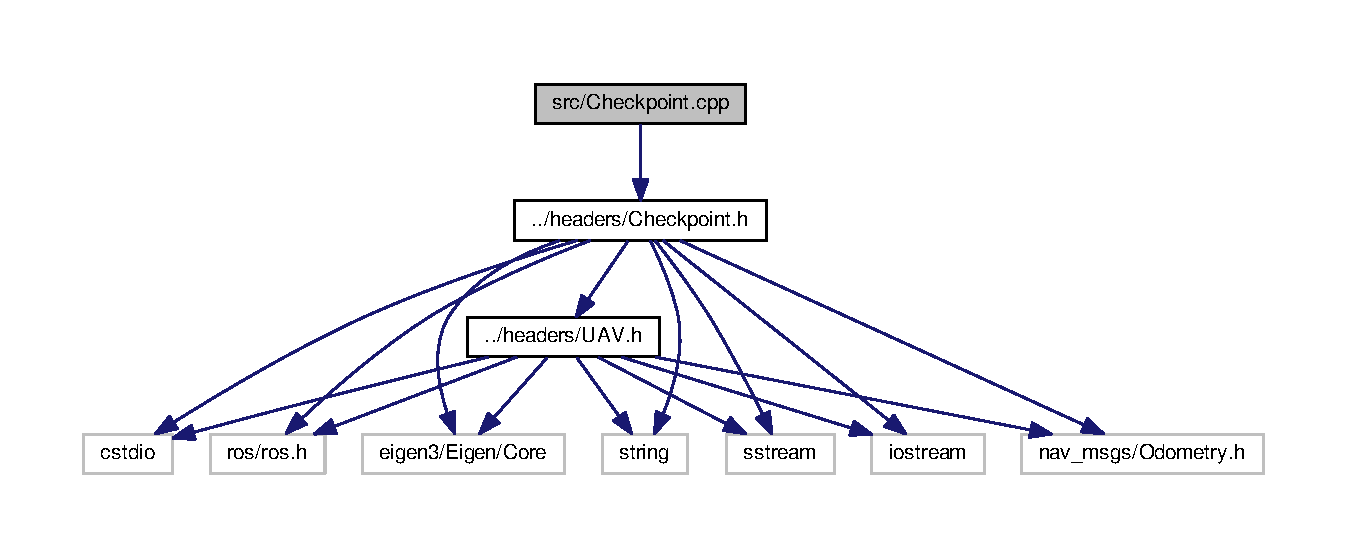
\includegraphics[width=350pt]{Checkpoint_8cpp__incl}
\end{center}
\end{figure}


\subsection{Detailed Description}
Contains definitions for the Checkpoints class. 

Contains function definitions for the \hyperlink{classCheckpoint}{Checkpoint} class. The \hyperlink{classCheckpoint}{Checkpoint} class consists of functions required for detecting that the \hyperlink{classUAV}{U\+AV} swarm has flown through a particular location and for measuring time of flight. 
\hypertarget{data__fitting_8cpp}{}\section{src/data\+\_\+fitting.cpp File Reference}
\label{data__fitting_8cpp}\index{src/data\+\_\+fitting.\+cpp@{src/data\+\_\+fitting.\+cpp}}


Contains functions required for evaluating the graph.  


{\ttfamily \#include \char`\"{}../headers/data\+\_\+fitting.\+h\char`\"{}}\\*
Include dependency graph for data\+\_\+fitting.\+cpp\+:\nopagebreak
\begin{figure}[H]
\begin{center}
\leavevmode
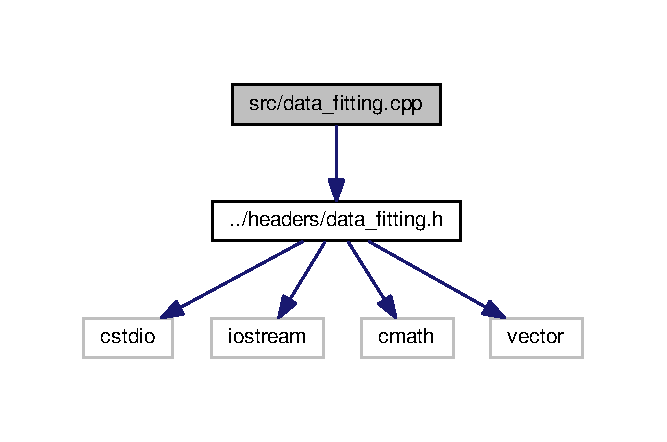
\includegraphics[width=320pt]{data__fitting_8cpp__incl}
\end{center}
\end{figure}
\subsection*{Functions}
\begin{DoxyCompactItemize}
\item 
void \hyperlink{data__fitting_8cpp_a74deb510fd707d8e6674b5dd45af6d31}{fitting\+\_\+run} (double time\+\_\+without\+\_\+obstacles, vector$<$ double $>$ x, vector$<$ vector$<$ double $>$$>$ y)
\item 
vector$<$ double $>$ \hyperlink{data__fitting_8cpp_a4527de60f484ec1a00df7164372d480a}{lin\+\_\+fit} (vector$<$ double $>$ x, vector$<$ double $>$ y)
\item 
vector$<$ double $>$ \hyperlink{data__fitting_8cpp_a375adde1de04ca6d8bae502b2902aa74}{exp\+\_\+fit} (vector$<$ double $>$ x, vector$<$ double $>$ y)
\end{DoxyCompactItemize}


\subsection{Detailed Description}
Contains functions required for evaluating the graph. 

Contains functions required for evaluating the graph using a heuristic function. 

\subsection{Function Documentation}
\index{data\+\_\+fitting.\+cpp@{data\+\_\+fitting.\+cpp}!exp\+\_\+fit@{exp\+\_\+fit}}
\index{exp\+\_\+fit@{exp\+\_\+fit}!data\+\_\+fitting.\+cpp@{data\+\_\+fitting.\+cpp}}
\subsubsection[{\texorpdfstring{exp\+\_\+fit(vector$<$ double $>$ x, vector$<$ double $>$ y)}{exp_fit(vector< double > x, vector< double > y)}}]{\setlength{\rightskip}{0pt plus 5cm}vector$<$double$>$ exp\+\_\+fit (
\begin{DoxyParamCaption}
\item[{vector$<$ double $>$}]{x, }
\item[{vector$<$ double $>$}]{y}
\end{DoxyParamCaption}
)}\hypertarget{data__fitting_8cpp_a375adde1de04ca6d8bae502b2902aa74}{}\label{data__fitting_8cpp_a375adde1de04ca6d8bae502b2902aa74}
Fits an exponential function to the input data 
\begin{DoxyParams}{Parameters}
{\em x} & X-\/axis of the input data \\
\hline
{\em y} & Y-\/axis of the input data \\
\hline
\end{DoxyParams}
\begin{DoxyReturn}{Returns}
std\+::vector$<$double$>$ of the exponential parameters (a,b) for f(x)=a$\ast$e$^\wedge$(b$\ast$x) 
\end{DoxyReturn}
\index{data\+\_\+fitting.\+cpp@{data\+\_\+fitting.\+cpp}!fitting\+\_\+run@{fitting\+\_\+run}}
\index{fitting\+\_\+run@{fitting\+\_\+run}!data\+\_\+fitting.\+cpp@{data\+\_\+fitting.\+cpp}}
\subsubsection[{\texorpdfstring{fitting\+\_\+run(double time\+\_\+without\+\_\+obstacles, vector$<$ double $>$ x, vector$<$ vector$<$ double $>$$>$ y)}{fitting_run(double time_without_obstacles, vector< double > x, vector< vector< double >> y)}}]{\setlength{\rightskip}{0pt plus 5cm}void fitting\+\_\+run (
\begin{DoxyParamCaption}
\item[{double}]{time\+\_\+without\+\_\+obstacles, }
\item[{vector$<$ double $>$}]{x, }
\item[{vector$<$ vector$<$ double $>$$>$}]{y}
\end{DoxyParamCaption}
)}\hypertarget{data__fitting_8cpp_a74deb510fd707d8e6674b5dd45af6d31}{}\label{data__fitting_8cpp_a74deb510fd707d8e6674b5dd45af6d31}
Computes the edges evaluation function and prints it out (d = distance, g = gap size, f = flock size) 
\begin{DoxyParams}{Parameters}
{\em time\+\_\+without\+\_\+obstacles} & measured time without obstacles normalized to 1 meter \\
\hline
{\em x} & x\mbox{[}i\mbox{]} = gap size for i-\/th measurement \\
\hline
{\em y} & y\mbox{[}F\+L\+O\+C\+K\+\_\+\+S\+I\+ZE\mbox{]}\mbox{[}i\mbox{]} = measured time increment for i-\/th gap size (normalized to 1 meter) \\
\hline
\end{DoxyParams}
\index{data\+\_\+fitting.\+cpp@{data\+\_\+fitting.\+cpp}!lin\+\_\+fit@{lin\+\_\+fit}}
\index{lin\+\_\+fit@{lin\+\_\+fit}!data\+\_\+fitting.\+cpp@{data\+\_\+fitting.\+cpp}}
\subsubsection[{\texorpdfstring{lin\+\_\+fit(vector$<$ double $>$ x, vector$<$ double $>$ y)}{lin_fit(vector< double > x, vector< double > y)}}]{\setlength{\rightskip}{0pt plus 5cm}vector$<$double$>$ lin\+\_\+fit (
\begin{DoxyParamCaption}
\item[{vector$<$ double $>$}]{x, }
\item[{vector$<$ double $>$}]{y}
\end{DoxyParamCaption}
)}\hypertarget{data__fitting_8cpp_a4527de60f484ec1a00df7164372d480a}{}\label{data__fitting_8cpp_a4527de60f484ec1a00df7164372d480a}
Fits a linear function to the input data 
\begin{DoxyParams}{Parameters}
{\em x} & X-\/axis of the input data \\
\hline
{\em y} & Y-\/axis of the input data \\
\hline
\end{DoxyParams}
\begin{DoxyReturn}{Returns}
std\+::vector$<$double$>$ of the exponential parameters (a,b) for f(x)=ax+b 
\end{DoxyReturn}

\hypertarget{graph_8cpp}{}\section{src/graph.cpp File Reference}
\label{graph_8cpp}\index{src/graph.\+cpp@{src/graph.\+cpp}}


Contains definitions of functions for representing the graph of paths and for path finding.  


{\ttfamily \#include \char`\"{}../headers/graph.\+h\char`\"{}}\\*
Include dependency graph for graph.\+cpp\+:\nopagebreak
\begin{figure}[H]
\begin{center}
\leavevmode
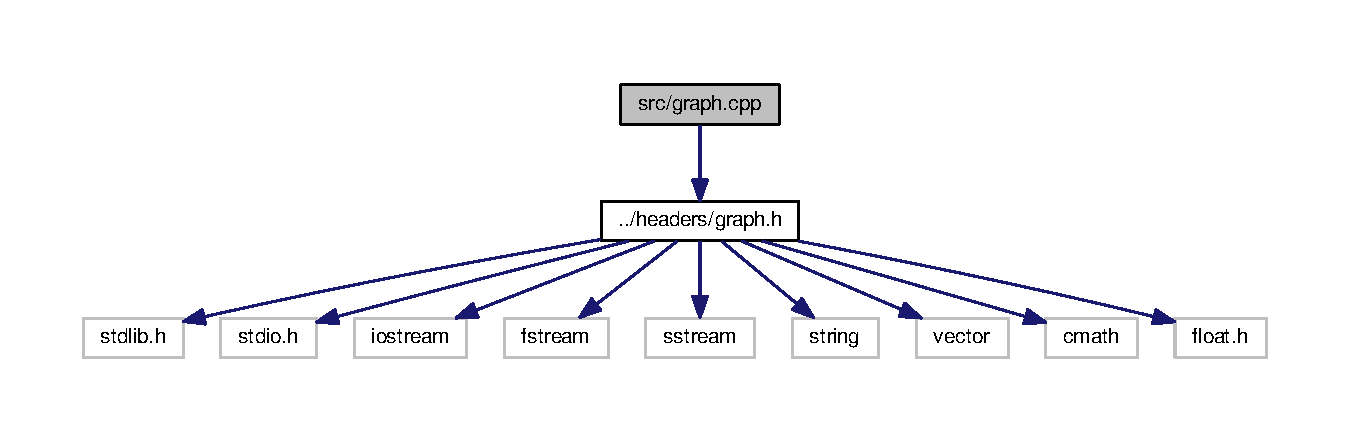
\includegraphics[width=350pt]{graph_8cpp__incl}
\end{center}
\end{figure}
\subsection*{Functions}
\begin{DoxyCompactItemize}
\item 
vector$<$ int $>$ \hyperlink{graph_8cpp_a4f76dec25df84647976b08cf172ab9b1}{find\+\_\+path} (const string \&fpath, int flock\+\_\+size, int source\+\_\+idx, int goal\+\_\+idx)
\item 
double \hyperlink{graph_8cpp_a9fba6aac78b4b7e5cddcc5c037ad6199}{evaluate\+\_\+edge} (vector$<$ double $>$ n1, vector$<$ double $>$ n2, int flock\+\_\+size, double gap)
\item 
int \hyperlink{graph_8cpp_a3fb0b3ab7cf6e09976ac5f8e075ade7a}{min\+Distance} (double dist\mbox{[}$\,$\mbox{]}, bool spt\+Set\mbox{[}$\,$\mbox{]}, unsigned long vnum)
\item 
vector$<$ int $>$ \hyperlink{graph_8cpp_a401501404aa387d4852fcc2a9ff3ad2d}{get\+\_\+path} (int parent\mbox{[}$\,$\mbox{]}, int j, vector$<$ int $>$ out)
\item 
vector$<$ int $>$ \hyperlink{graph_8cpp_a7f0876063956a2c9f083434f30d8abd3}{dijkstra} (vector$<$ vector$<$ double $>$$>$ graph, int src, int goal, unsigned long vnum)
\item 
vector$<$ vector$<$ double $>$ $>$ \hyperlink{graph_8cpp_ac83a486cf316213a12cbffd5598b2fdd}{load\+\_\+vertices} (const string \&path)
\item 
vector$<$ vector$<$ int $>$ $>$ \hyperlink{graph_8cpp_a5061393c1ae1c9773903ae2ac46adc0a}{load\+\_\+edges} (const string \&path)
\item 
vector$<$ string $>$ \hyperlink{graph_8cpp_a21228818f6b97bdd706d7980b74a2966}{split} (const string \&s)
\end{DoxyCompactItemize}


\subsection{Detailed Description}
Contains definitions of functions for representing the graph of paths and for path finding. 



\subsection{Function Documentation}
\index{graph.\+cpp@{graph.\+cpp}!dijkstra@{dijkstra}}
\index{dijkstra@{dijkstra}!graph.\+cpp@{graph.\+cpp}}
\subsubsection[{\texorpdfstring{dijkstra(vector$<$ vector$<$ double $>$$>$ graph, int src, int goal, unsigned long vnum)}{dijkstra(vector< vector< double >> graph, int src, int goal, unsigned long vnum)}}]{\setlength{\rightskip}{0pt plus 5cm}vector$<$int$>$ dijkstra (
\begin{DoxyParamCaption}
\item[{vector$<$ vector$<$ double $>$$>$}]{graph, }
\item[{int}]{src, }
\item[{int}]{goal, }
\item[{unsigned long}]{vnum}
\end{DoxyParamCaption}
)}\hypertarget{graph_8cpp_a7f0876063956a2c9f083434f30d8abd3}{}\label{graph_8cpp_a7f0876063956a2c9f083434f30d8abd3}
Dijkstra\textquotesingle{}s single source algorithm for a graph represented using adjacency matrix 
\begin{DoxyParams}{Parameters}
{\em graph} & graph representation \\
\hline
{\em src} & source node index \\
\hline
{\em vnum} & number of vertices in the graph \\
\hline
\end{DoxyParams}
\index{graph.\+cpp@{graph.\+cpp}!evaluate\+\_\+edge@{evaluate\+\_\+edge}}
\index{evaluate\+\_\+edge@{evaluate\+\_\+edge}!graph.\+cpp@{graph.\+cpp}}
\subsubsection[{\texorpdfstring{evaluate\+\_\+edge(vector$<$ double $>$ n1, vector$<$ double $>$ n2, int flock\+\_\+size, double gap)}{evaluate_edge(vector< double > n1, vector< double > n2, int flock_size, double gap)}}]{\setlength{\rightskip}{0pt plus 5cm}double evaluate\+\_\+edge (
\begin{DoxyParamCaption}
\item[{vector$<$ double $>$}]{n1, }
\item[{vector$<$ double $>$}]{n2, }
\item[{int}]{flock\+\_\+size, }
\item[{double}]{gap}
\end{DoxyParamCaption}
)}\hypertarget{graph_8cpp_a9fba6aac78b4b7e5cddcc5c037ad6199}{}\label{graph_8cpp_a9fba6aac78b4b7e5cddcc5c037ad6199}
Evaluates graph edge 
\begin{DoxyParams}{Parameters}
{\em n1} & node \#1 coordinates \\
\hline
{\em n2} & node \#2 coordinates \\
\hline
{\em flock\+\_\+size} & number of U\+A\+Vs \\
\hline
{\em gap} & size of gap between obstacles around the edge \\
\hline
\end{DoxyParams}
\begin{DoxyReturn}{Returns}
edge cost 
\end{DoxyReturn}
\index{graph.\+cpp@{graph.\+cpp}!find\+\_\+path@{find\+\_\+path}}
\index{find\+\_\+path@{find\+\_\+path}!graph.\+cpp@{graph.\+cpp}}
\subsubsection[{\texorpdfstring{find\+\_\+path(const string \&fpath, int flock\+\_\+size, int source\+\_\+idx, int goal\+\_\+idx)}{find_path(const string &fpath, int flock_size, int source_idx, int goal_idx)}}]{\setlength{\rightskip}{0pt plus 5cm}vector$<$int$>$ find\+\_\+path (
\begin{DoxyParamCaption}
\item[{const string \&}]{fpath, }
\item[{int}]{flock\+\_\+size, }
\item[{int}]{source\+\_\+idx, }
\item[{int}]{goal\+\_\+idx}
\end{DoxyParamCaption}
)}\hypertarget{graph_8cpp_a4f76dec25df84647976b08cf172ab9b1}{}\label{graph_8cpp_a4f76dec25df84647976b08cf172ab9b1}
Main path finding function -\/ loads graph and finds the shortest path from the start node to the end node 
\begin{DoxyParams}{Parameters}
{\em fpath} & graph file path \\
\hline
{\em flock\+\_\+size} & number of U\+A\+Vs \\
\hline
{\em source\+\_\+idx} & start node \\
\hline
{\em goal\+\_\+idx} & end node \\
\hline
\end{DoxyParams}
\begin{DoxyReturn}{Returns}
path as a vector of node indices 
\end{DoxyReturn}
\index{graph.\+cpp@{graph.\+cpp}!get\+\_\+path@{get\+\_\+path}}
\index{get\+\_\+path@{get\+\_\+path}!graph.\+cpp@{graph.\+cpp}}
\subsubsection[{\texorpdfstring{get\+\_\+path(int parent[], int j, vector$<$ int $>$ out)}{get_path(int parent[], int j, vector< int > out)}}]{\setlength{\rightskip}{0pt plus 5cm}vector$<$int$>$ get\+\_\+path (
\begin{DoxyParamCaption}
\item[{int}]{parent\mbox{[}$\,$\mbox{]}, }
\item[{int}]{j, }
\item[{vector$<$ int $>$}]{out}
\end{DoxyParamCaption}
)}\hypertarget{graph_8cpp_a401501404aa387d4852fcc2a9ff3ad2d}{}\label{graph_8cpp_a401501404aa387d4852fcc2a9ff3ad2d}
Function to find shortest path from source to j using parent array 
\begin{DoxyParams}{Parameters}
{\em parent} & parent node array \\
\hline
{\em j} & goal node \\
\hline
\end{DoxyParams}
\index{graph.\+cpp@{graph.\+cpp}!load\+\_\+edges@{load\+\_\+edges}}
\index{load\+\_\+edges@{load\+\_\+edges}!graph.\+cpp@{graph.\+cpp}}
\subsubsection[{\texorpdfstring{load\+\_\+edges(const string \&path)}{load_edges(const string &path)}}]{\setlength{\rightskip}{0pt plus 5cm}vector$<$vector$<$int$>$ $>$ load\+\_\+edges (
\begin{DoxyParamCaption}
\item[{const string \&}]{path}
\end{DoxyParamCaption}
)}\hypertarget{graph_8cpp_a5061393c1ae1c9773903ae2ac46adc0a}{}\label{graph_8cpp_a5061393c1ae1c9773903ae2ac46adc0a}
Loads edges from the given file 
\begin{DoxyParams}{Parameters}
{\em path} & file path \\
\hline
\end{DoxyParams}
\begin{DoxyReturn}{Returns}
edges as vertex indices 
\end{DoxyReturn}
\index{graph.\+cpp@{graph.\+cpp}!load\+\_\+vertices@{load\+\_\+vertices}}
\index{load\+\_\+vertices@{load\+\_\+vertices}!graph.\+cpp@{graph.\+cpp}}
\subsubsection[{\texorpdfstring{load\+\_\+vertices(const string \&path)}{load_vertices(const string &path)}}]{\setlength{\rightskip}{0pt plus 5cm}vector$<$vector$<$double$>$ $>$ load\+\_\+vertices (
\begin{DoxyParamCaption}
\item[{const string \&}]{path}
\end{DoxyParamCaption}
)}\hypertarget{graph_8cpp_ac83a486cf316213a12cbffd5598b2fdd}{}\label{graph_8cpp_ac83a486cf316213a12cbffd5598b2fdd}
Loads vertices from the given file (+converts mm to m) 
\begin{DoxyParams}{Parameters}
{\em path} & file path \\
\hline
\end{DoxyParams}
\begin{DoxyReturn}{Returns}
vertices coordinates 
\end{DoxyReturn}
\index{graph.\+cpp@{graph.\+cpp}!min\+Distance@{min\+Distance}}
\index{min\+Distance@{min\+Distance}!graph.\+cpp@{graph.\+cpp}}
\subsubsection[{\texorpdfstring{min\+Distance(double dist[], bool spt\+Set[], unsigned long vnum)}{minDistance(double dist[], bool sptSet[], unsigned long vnum)}}]{\setlength{\rightskip}{0pt plus 5cm}int min\+Distance (
\begin{DoxyParamCaption}
\item[{double}]{dist\mbox{[}$\,$\mbox{]}, }
\item[{bool}]{spt\+Set\mbox{[}$\,$\mbox{]}, }
\item[{unsigned long}]{vnum}
\end{DoxyParamCaption}
)}\hypertarget{graph_8cpp_a3fb0b3ab7cf6e09976ac5f8e075ade7a}{}\label{graph_8cpp_a3fb0b3ab7cf6e09976ac5f8e075ade7a}
A utility function to find the vertex with minimum distance value, from the set of vertices not yet included in shortest path tree 
\begin{DoxyParams}{Parameters}
{\em dist} & dist\mbox{[}i\mbox{]} = the shortest distance from src to i \\
\hline
{\em spt\+Set} & spt\+Set\mbox{[}i\mbox{]} = true if vertex i is included or in shortest path tree or shortest distance from src to i is finalized \\
\hline
{\em vnum} & number of vertices in the graph \\
\hline
\end{DoxyParams}
\begin{DoxyReturn}{Returns}
index of closest vertex 
\end{DoxyReturn}
\index{graph.\+cpp@{graph.\+cpp}!split@{split}}
\index{split@{split}!graph.\+cpp@{graph.\+cpp}}
\subsubsection[{\texorpdfstring{split(const string \&s)}{split(const string &s)}}]{\setlength{\rightskip}{0pt plus 5cm}vector$<$string$>$ split (
\begin{DoxyParamCaption}
\item[{const string \&}]{s}
\end{DoxyParamCaption}
)}\hypertarget{graph_8cpp_a21228818f6b97bdd706d7980b74a2966}{}\label{graph_8cpp_a21228818f6b97bdd706d7980b74a2966}
Utility function for string splitting using spaces as delimiter 
\begin{DoxyParams}{Parameters}
{\em s} & input string \\
\hline
\end{DoxyParams}
\begin{DoxyReturn}{Returns}
vector of words 
\end{DoxyReturn}

\hypertarget{UAV_8cpp}{}\section{src/\+U\+AV.cpp File Reference}
\label{UAV_8cpp}\index{src/\+U\+A\+V.\+cpp@{src/\+U\+A\+V.\+cpp}}


Class for representing the \hyperlink{classUAV}{U\+AV}.  


{\ttfamily \#include \char`\"{}../headers/\+U\+A\+V.\+h\char`\"{}}\\*
Include dependency graph for U\+A\+V.\+cpp\+:
\nopagebreak
\begin{figure}[H]
\begin{center}
\leavevmode
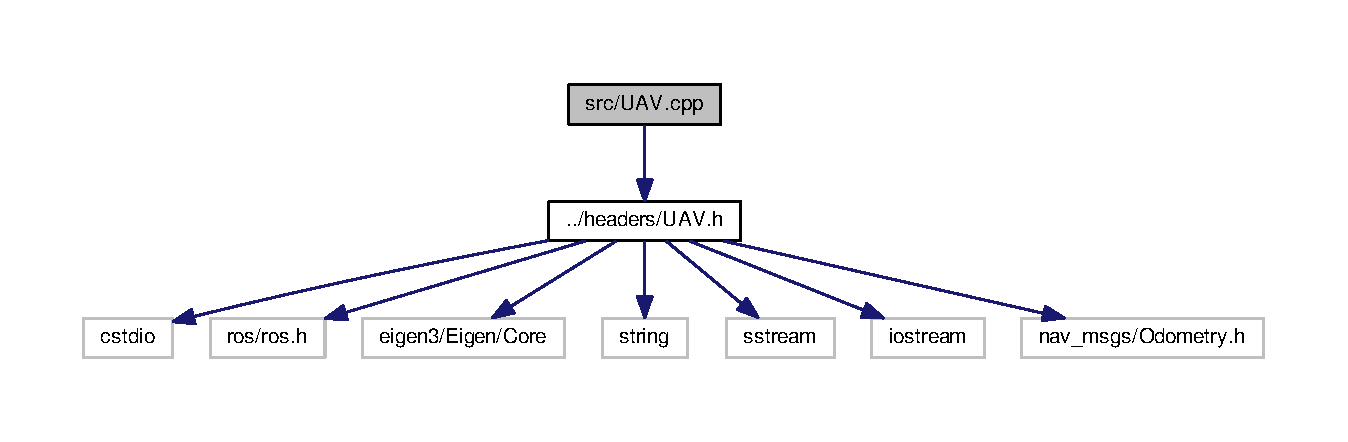
\includegraphics[width=350pt]{UAV_8cpp__incl}
\end{center}
\end{figure}


\subsection{Detailed Description}
Class for representing the \hyperlink{classUAV}{U\+AV}. 

Contains function definitions for the \hyperlink{classUAV}{U\+AV} class. The \hyperlink{classUAV}{U\+AV} class consists of location callback for updating the \hyperlink{classUAV}{U\+AV} location. 
%--- End generated contents ---

% Index
\backmatter
\newpage
\phantomsection
\clearemptydoublepage
\addcontentsline{toc}{chapter}{Index}
\printindex

\end{document}
